\chapter{Interactive Data Exploration Applications}\label{interactive}
% why care for explorative 
Visualization is central in both the analysis and understanding of biological
functions in high-throughput biological
datasets.\cite{gehlenborg2010visualization} Because of the complexity of
the biological data and analyses, we need specialized software to analyze and
generate understandable visual representations of the complex datasets.\cite{o2018visualization} 
While more tools are becoming available, application developers still
face multiple challenges when designing these
tools.\cite{o2018visualization,o2010visualizing} In addition to visualizing the
relevant data, tools often integrate with online databases to allow researchers
to study the data in the context of previous
knowledge.\cite{gehlenborg2010visualization,o2018visualization}

Data analysis tools in systems biology are greatly reliant on programming
languages specially tailored to these domains.\cite{fjukstad2017building}
Languages such as Python or R both provide a wealth of statistical packages and
frameworks.  However, these specialized programming environments often do not
provide interactive interfaces for researchers that want to explore the results
from the analyses without using a programmatic interface. Frameworks such as
Shiny\cite{shiny} and OpenCPU\cite{opencpu} allow application developers to
build systems to interactively explore results from statistical analyses in R.
These systems can then provide understandable graphical user interfaces on top
of complex statistical software that require programming skills to navigate.  To
interpret data, experts regularly exploit prior knowledge via database queries
and the primary scientific literature. There are a wealth of online databases,
some of which provide open \glspl{api} in addition to web user interfaces that
application developers can make use of. For visually exploring biological data
there are a range of tools, such as Cytoscape\cite{cytoscape} and
Circos\cite{circos}, that support importing an already-analyzed dataset to
visualize and browse the data. One problem with these are that they are
decoupled from the analysis, making it difficult to retrace the data processing
prior to the end results.  

One of the main issues for developing these types of data exploration
applications is that they require the integration of disparate systems and
tools. The datasets require specialized analysis software, often with large
computational resources, and the end users require simple point-and-click
interface available on their device. In addition it is crucial for
reproducibility to keep track of the data processing steps that were used to
generate end visualizations. 

We have developed two data exploration applications, Kvik
Pathways\cite{fjukstad2015kvik} and
MIxT\cite{fjukstad2017building,dumeaux2017interactions} for exploring
transcriptional profiles in the \gls{nowac} study through interactive
visualizations integrated with biological databases. We first developed Kvik
Pathways to explore transcriptional profiles in the context of biological
pathway maps. It is a three-tiered web application consisting of three central
components, that we later refactored into three separate microservices for use
in other applications. These three microservices make up the \glspl{sme} in our
approach for building data exploration applications.  With these microservices
we implemented the MIxT web application, and generalized our efforts into
general design principles for data exploration applications.  While our
applications provide specialized user interfaces, we show how the design
patterns and ideas can be used in a wide range of use cases. We also provide an
evaluation that shows that our approach is suitable for this type of interactive
applications. 

This chapter is based on Papers 1 and 2, as well as the general descriptions of
the MIxT system in Paper 3. 
The rest of the chapter is organized as follows: First we present the two
motivating use cases for our applications. We then detail the requirements for
these types of interactive applications. Following the requirements we detail
the Kvik Pathways application, including its architecture and implementation. We
then show how we use this first application to generalize its design principle
and show we can use them to build applications that follow the \gls{sme}
approach. Following is a description of the implementation of the \glspl{sme}
approach in the microservices in Kvik. We present how we used these to develop
the MIxT web application. Finally we discuss our approach in context of related
work, and provide a conclusion. 

\section{Motivating Use Cases}
The need for interactive applications has come from two different previous
projects in the \gls{nowac} study. Both of these rely on advanced statistical
analyses and produce comprehensive results that are interpreted by researchers
in the context of related information from online biological databases. The end
results from the statistical analyses are typically large tables that require
manual inspection and linking with known biology. Below we describe the two
applications before we detail the requirements, design and implementation of the
applications.

\subsection{High and Low Plasma Ratios of Essential Fatty Acids} 
The aim of the first application was a to explore the results from a previous
published project that compared gene expression in blood from healthy women with
high and low plasma ratios of essential fatty acids.\cite{olsen2013plasma}  Gene
expression differences where assessed and determined that there were 184
differentially expressed genes. When exploring this list of 184 genes,
functional information was retrieved from GeneCards and other repositories, and
the list was analyzed for overlap with known pathways using MSigDB
\footnote{Available online at
\href{broadinstitute.org/gsea/msigdb}{broadinstitute.org/gsea/msigdb}}. The
researchers had to manually maintain overview of single genes, gene networks or
pathways, and gather functional information gene by gene while assessing
differences in gene expression levels. With this approach, researchers were
limited by their own capacity to retrieve information manually from databases
and keep it up to date. An application could automate the retrieval and ensure
that the data is correct and up to date. 

\subsection{Tumor-Blood Interactions in Breast Cancer Patients}
The aim of the Matched Interactions Across Tissues (MIxT) study was to identify
genes and pathways in the primary breast tumor that are tightly linked to genes
and pathways in the patient blood cells.\cite{dumeaux2017interactions} We
generated and analyzed expression profiles from blood and matched tumor cells in
173 breast cancer patients included in the \gls{nowac} 
study.  The MIxT analysis starts by identifying sets of genes tightly
co-expressed across all patients in each tissue. Each group of genes or modules
were annotated based on a priori biological knowledge about gene functionality.
Then the analyses investigate the relationships between tissues by asking if
specific biologies in one tissue are linked with (possibly distinct) biologies
in the second tissue, and this within different subgroup of patients (i.e.
subtypes of breast cancer).

\section{Requirements} 
From these two studies we identified a set of requirements that the data
exploration applications should satisfy. These are all based on the needs of the
researchers in the \gls{nowac} study. 

\begin{description} 
\item[Interactive] The applications should provide interactive exploration
    of datasets through visualizations and integration with relevant
    information.
    
\item[Familiar] The applications should use familiar visual representations to
    present information to researchers. By using familiar or intuitive
        conventions we can reduce the cognitive load needed to read a
        visualization and gain insight from it.\cite{o2018visualization}
    
\item[Simple to use] Researchers should not need to install software to
    explore their data through the applications. The applications should 
    protect the researcher from the burden of installing and keeping an
    application up to date. 
    
\item[Lightweight] Data presentation and computation should be separated
    to make it possible for researchers to explore data without having to
    have the computational power to run the analyses. With the growing rate
    data is produced at, we cannot expect that researchers have the resources to
    store and analyze data on their own computers. 
    
\end{description}

With these requirements in mind we set out to develop two applications for
interactively explore the results from the studies along with information
from online databases. 

\section{Kvik Pathways}
The first application we developed was Kvik Pathways. Kvik Pathways allows users
to interactively explore a molecular dataset, such as gene expression, through a
web application.\cite{fjukstad2015kvik} It provides pathway visualizations and
detailed information about genes and pathways from the KEGG database. Figure
\ref{kvikpwfig} shows a screenshot of the user interface of Kvik Pathways.
Through pathway visualizations and integration with the KEGG databases, users
can perform targeted exploration of pathways and genes to get an overview of the
biological functions that are involved with gene expression from the underlying
dataset.  Kvik Pathways gathers information about related pathways and retrieves
relevant information about genes, making it unnecessary for researchers to spend
valuable time looking up this information manually. Previously researchers had
to manually retrieve information from \gls{kegg} while browsing pathway maps,
interrupting the visual analysis process.  Kvik Pathways retrieves information
about genes without the researcher having to leave the pathway visualization to
retrieve relevant information.

\subsection{Analysis Tasks} 
To efficiently develop the application we designed 3 analysis tasks that the
application supports. 

\textbf{A1:} Explore gene expression in the context of \gls{kegg} pathway maps.
It provides users with a list of pathway maps to choose from, and the
application will generate an interactive visualization including gene expression
values. 

\textbf{A2:} Investigate and retrieve relevant biological information. It
provides users with direct links to online databases with up to date
information. 

\textbf{A3:} Explore relationships between pathway maps. When users select a
gene from a pathway map they get a list of other pathway maps that this gene is
found in, in addition to their similarity. This allows users to investigate the
biological processes the genes are a part of. 

\begin{figure}[htb!]
    \begin{centering}
    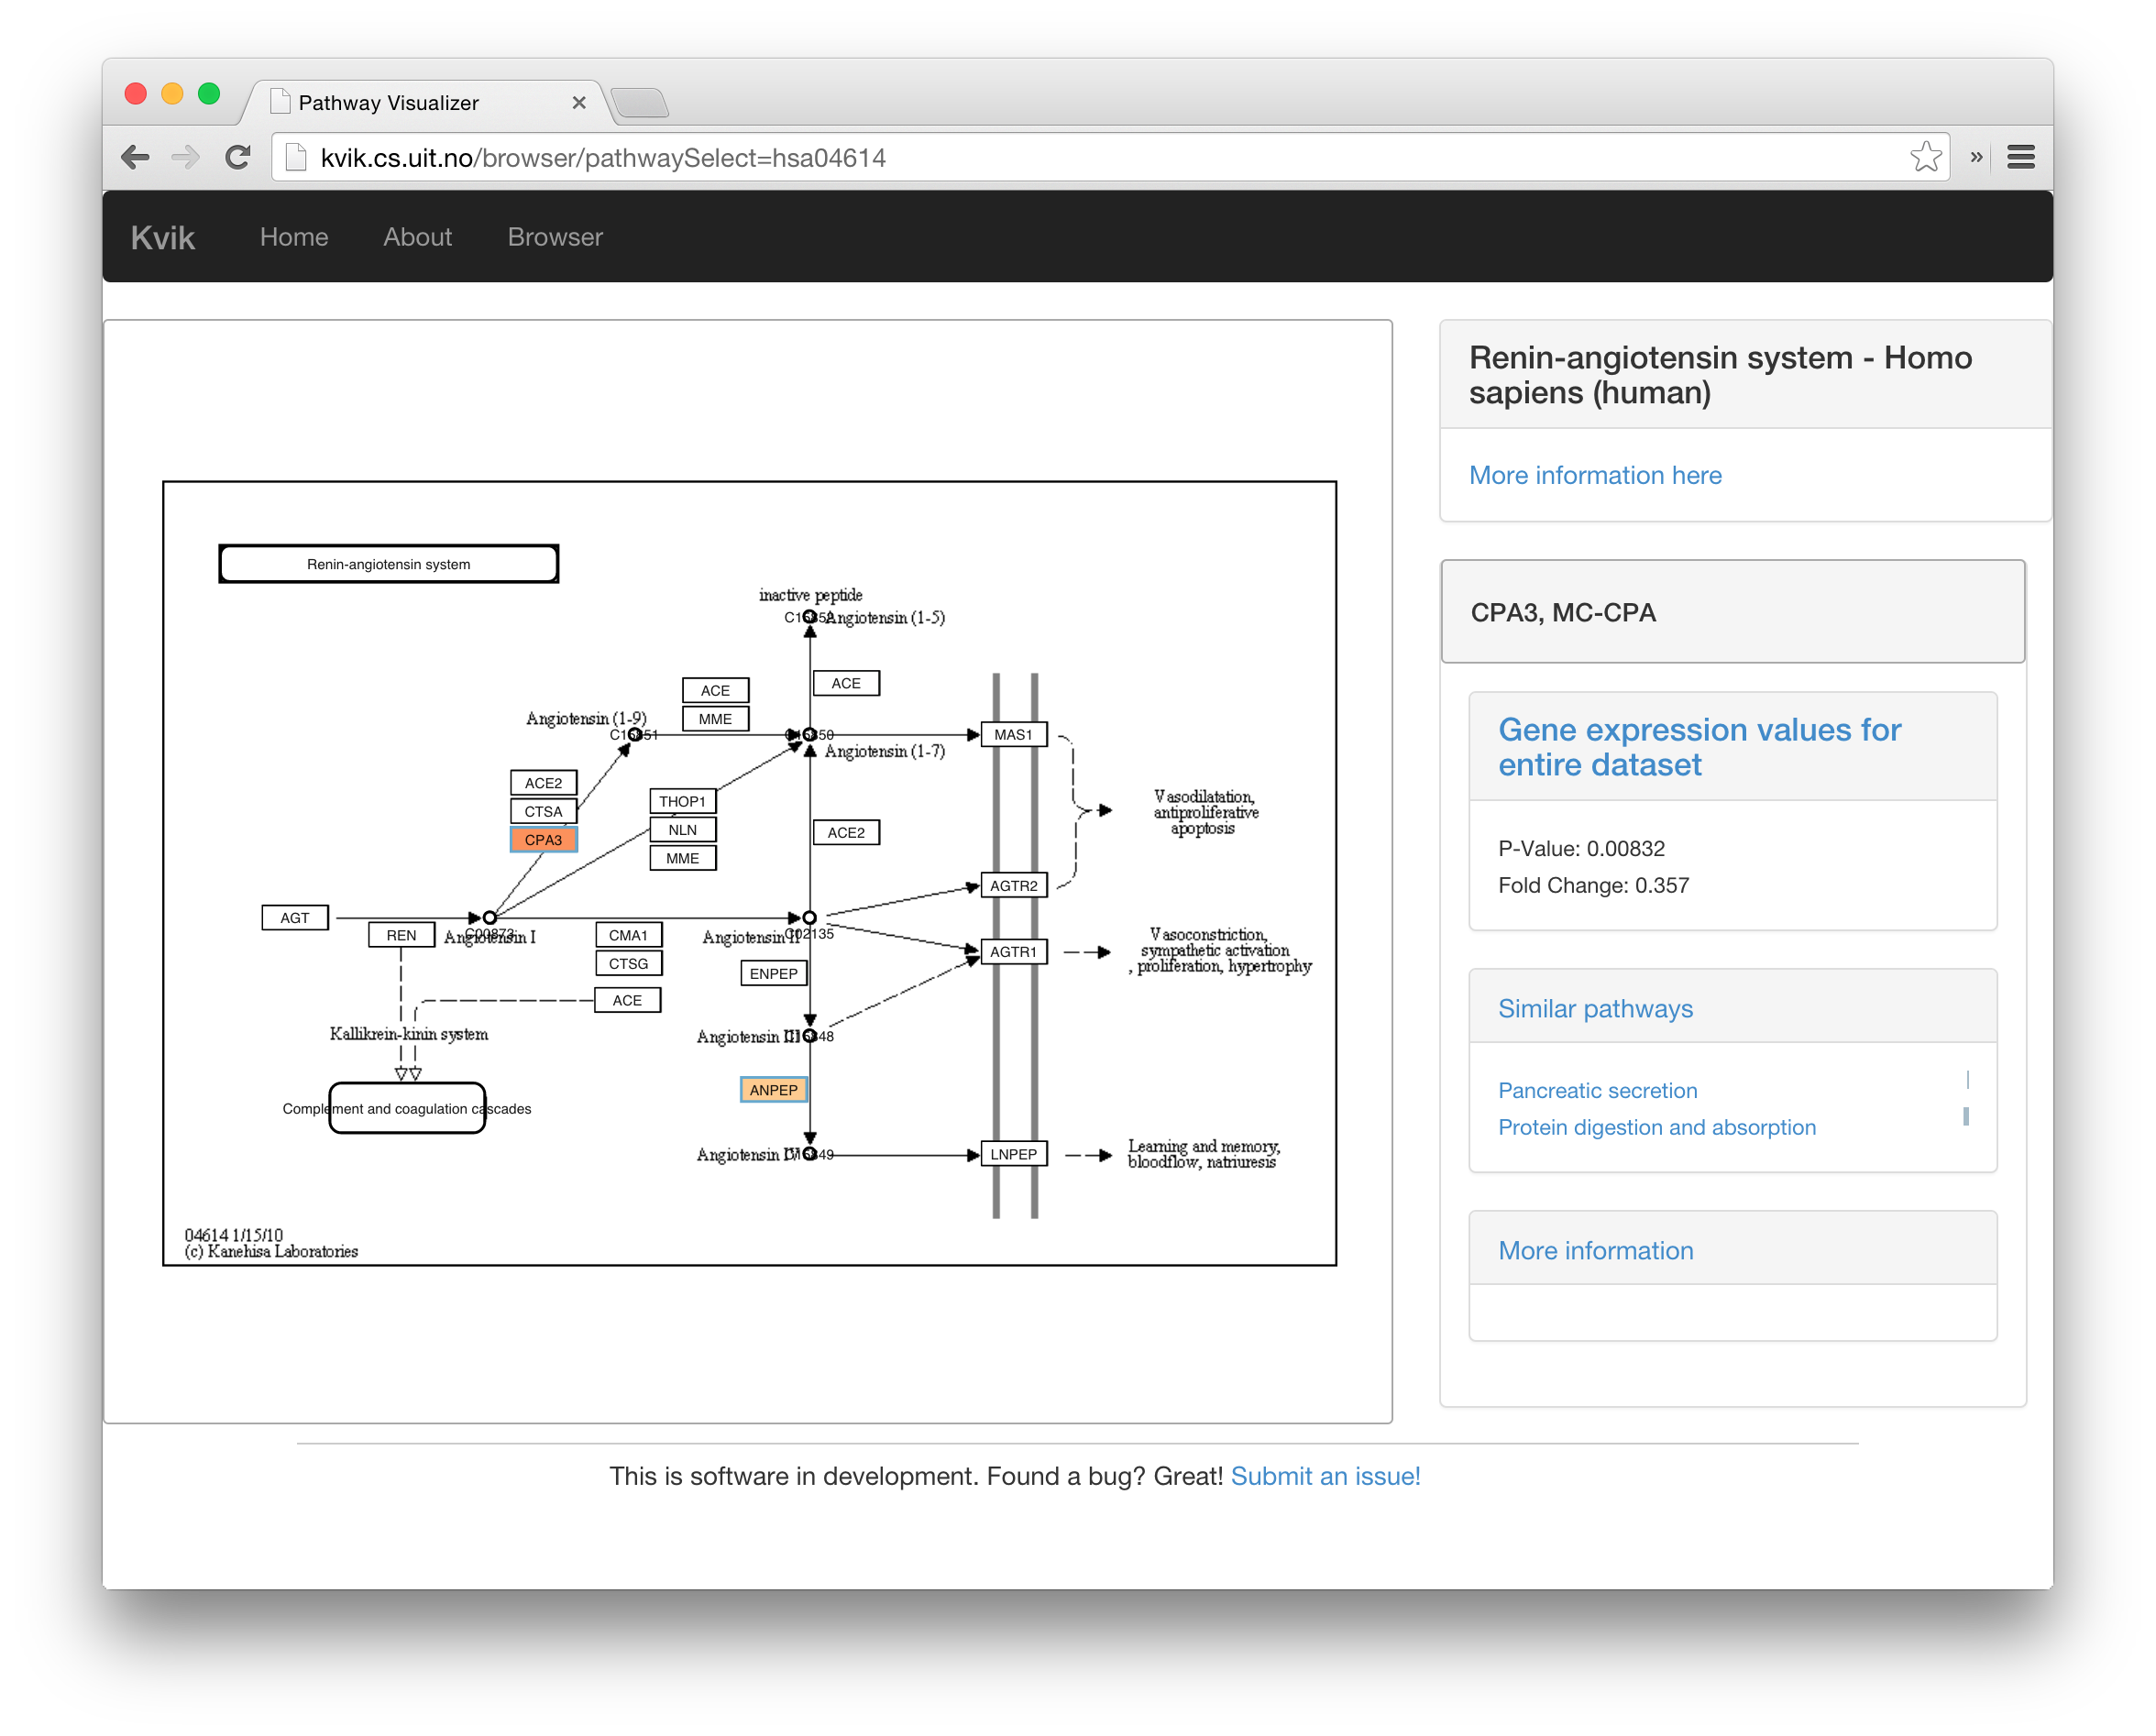
\includegraphics[width=\textwidth]{figures/kvikpwfig.png}
        \caption[Screenshot of the renin-angiotensin pathway in Kvik
        Pathways]{Screenshot of the renin-angiotensin pathway (KEGG pathway id
        hsa04614) in Kvik Pathways. Researchers can visually explore the
        pathways and read relevant information about genes in the right-hand
        panel.}
    \label{kvikpwfig}
    \end{centering} 
\end{figure}


\subsection{Architecture} 
Kvik Pathways has a three-tiered architecture of independent layers (Figure
\ref{fig:arch}). The browser layer consists of the web application for
exploring gene expression data and biological pathways. A front-end layer
provides static content such as HTML pages and stylesheets, as well as an
interface to the data sources with dynamic content such as gene expression
data or pathway maps to the web application. The backend layer contains
information about pathways and genes, as well as computational and storage
resources to process genomic data such as the \gls{nowac}  data repository. We
have used the packages in Kvik to develop the backend layer. These are discissed
in detail in Section \ref{kviksec}. 

The Data Engine in the backend layer provides an interface to the \gls{nowac}
data repository stored on a secure server on our local supercomputer. In Kvik
Pathways all gene expression data is stored on the computer that runs the Data
Engine. The Data Engine runs an R session accessible over remote procedure calls
(RPCs) from the front-end layer using RPy2\cite{rpy2} to interface with R. To
access data and run analyses the Data Interface exposes a HTTP \gls{api} to the
browser layer (Table \ref{interfacetable} provides the interfaces).

\begin{figure}[htb]
    \begin{centering}
    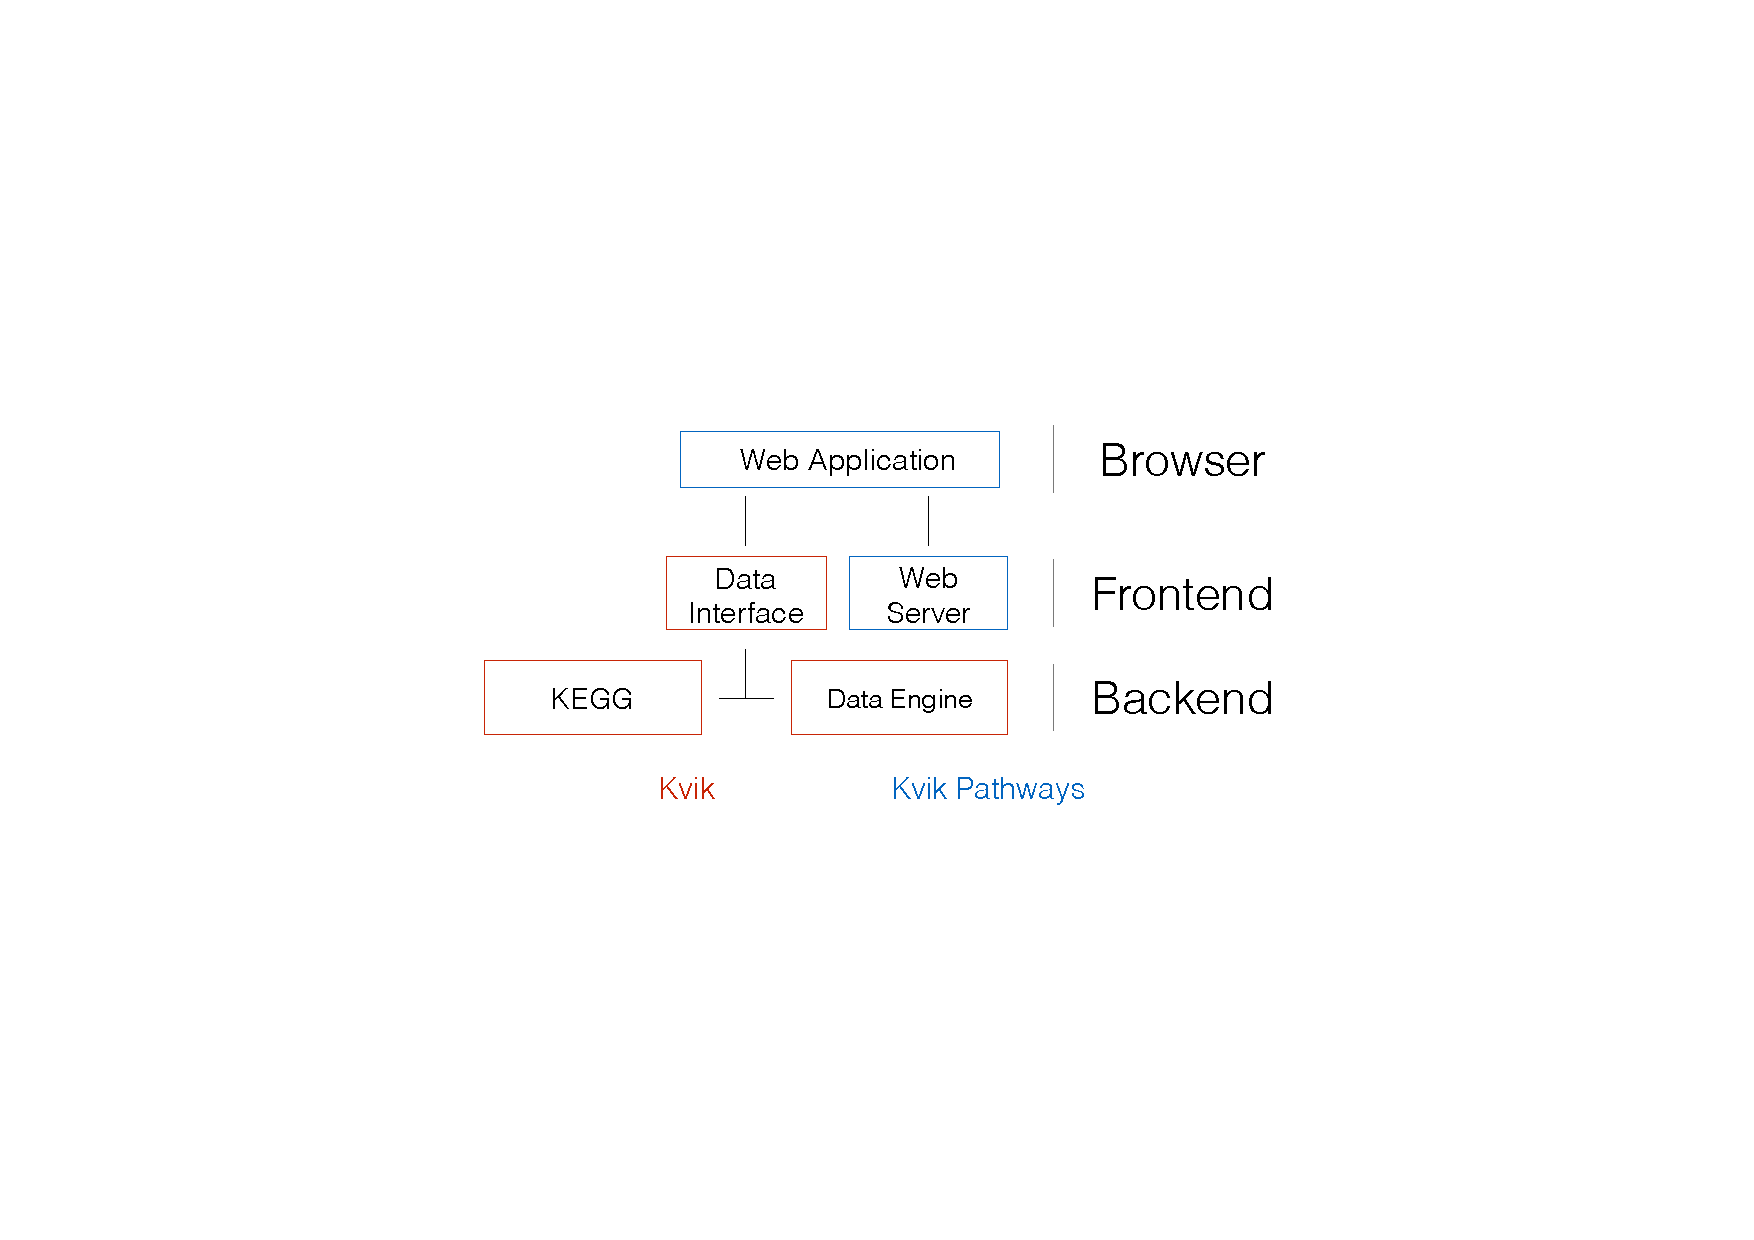
\includegraphics[width=\textwidth]{figures/archv2-name-fix.pdf}
    \caption{The three-tiered architecture of Kvik Pathways.} 
    \label{fig:arch}
    \end{centering} 
\end{figure}   

\begin{table}[!t]
\renewcommand{\arraystretch}{1.3}
\caption{
The REST interface to the Data Engine. For example, use \texttt{/genes/} to
    retrieve all available genes in our dataset.
}
\label{t1}
\centering\small
\begin{tabular*}{\linewidth}{@{\extracolsep{\fill}}p{0.025\linewidth}p{0.7\linewidth}@{}}
\hline
\bfseries URL & \bfseries Description\\
\hline
\emph{/fc/[genes...]} & Calculate and retrieve fold-change for the specified
    genes \\
\emph{/pvalues/[genes...]} & Calculate and retrieve $p$-values for the specified
    genes\\
\emph{/exprs/[genes...]} & Get the raw gene expression values from the dataset
    \\
\emph{/genes} & Get a list of all genes in the dataset \\
\hline
\end{tabular*}
    \label{interfacetable}
\end{table}

\subsection{Implementation} 
To create pathway visualizations the Kvik backend retrieves and parses the KEGG
Markup Language (KGML) representation and pathway image from KEGG databases
through its REST \gls{api}.\cite{kgml} This KGML representation of a pathway is an XML
file that contains a list of nodes (genes, proteins or compounds) and edges
(reactions or relations). Kvik parses this file and generates a JSON
representation that Kvik Pathway uses to create pathway visualizations.  Kvik
Pathways uses Cytoscape.js\cite{cytoscapejs} to create a pathway visualization
from the list of nodes and edges and overlay the nodes on the pathway image. See
Figure \ref{fig:how2pathway} for a graphical illustration of the process. To
reduce latency when using the \gls{kegg} \gls{rest} \gls{api}, we cache every
response on our servers.  We use the average fold change between the groups
(women with high or low plasma ratios of essential fatty acids) in the dataset
to color the genes within the pathway maps.  To highlight $p$-values, the
pathway visualization shows an additional colored frame around genes. We
visualize fold change values for individual samples as a bar chart in a side
panel.  This bar chart gives researchers a global view of the fold change in the
entire dataset. 

\begin{figure}[htb]
    \begin{centering}
    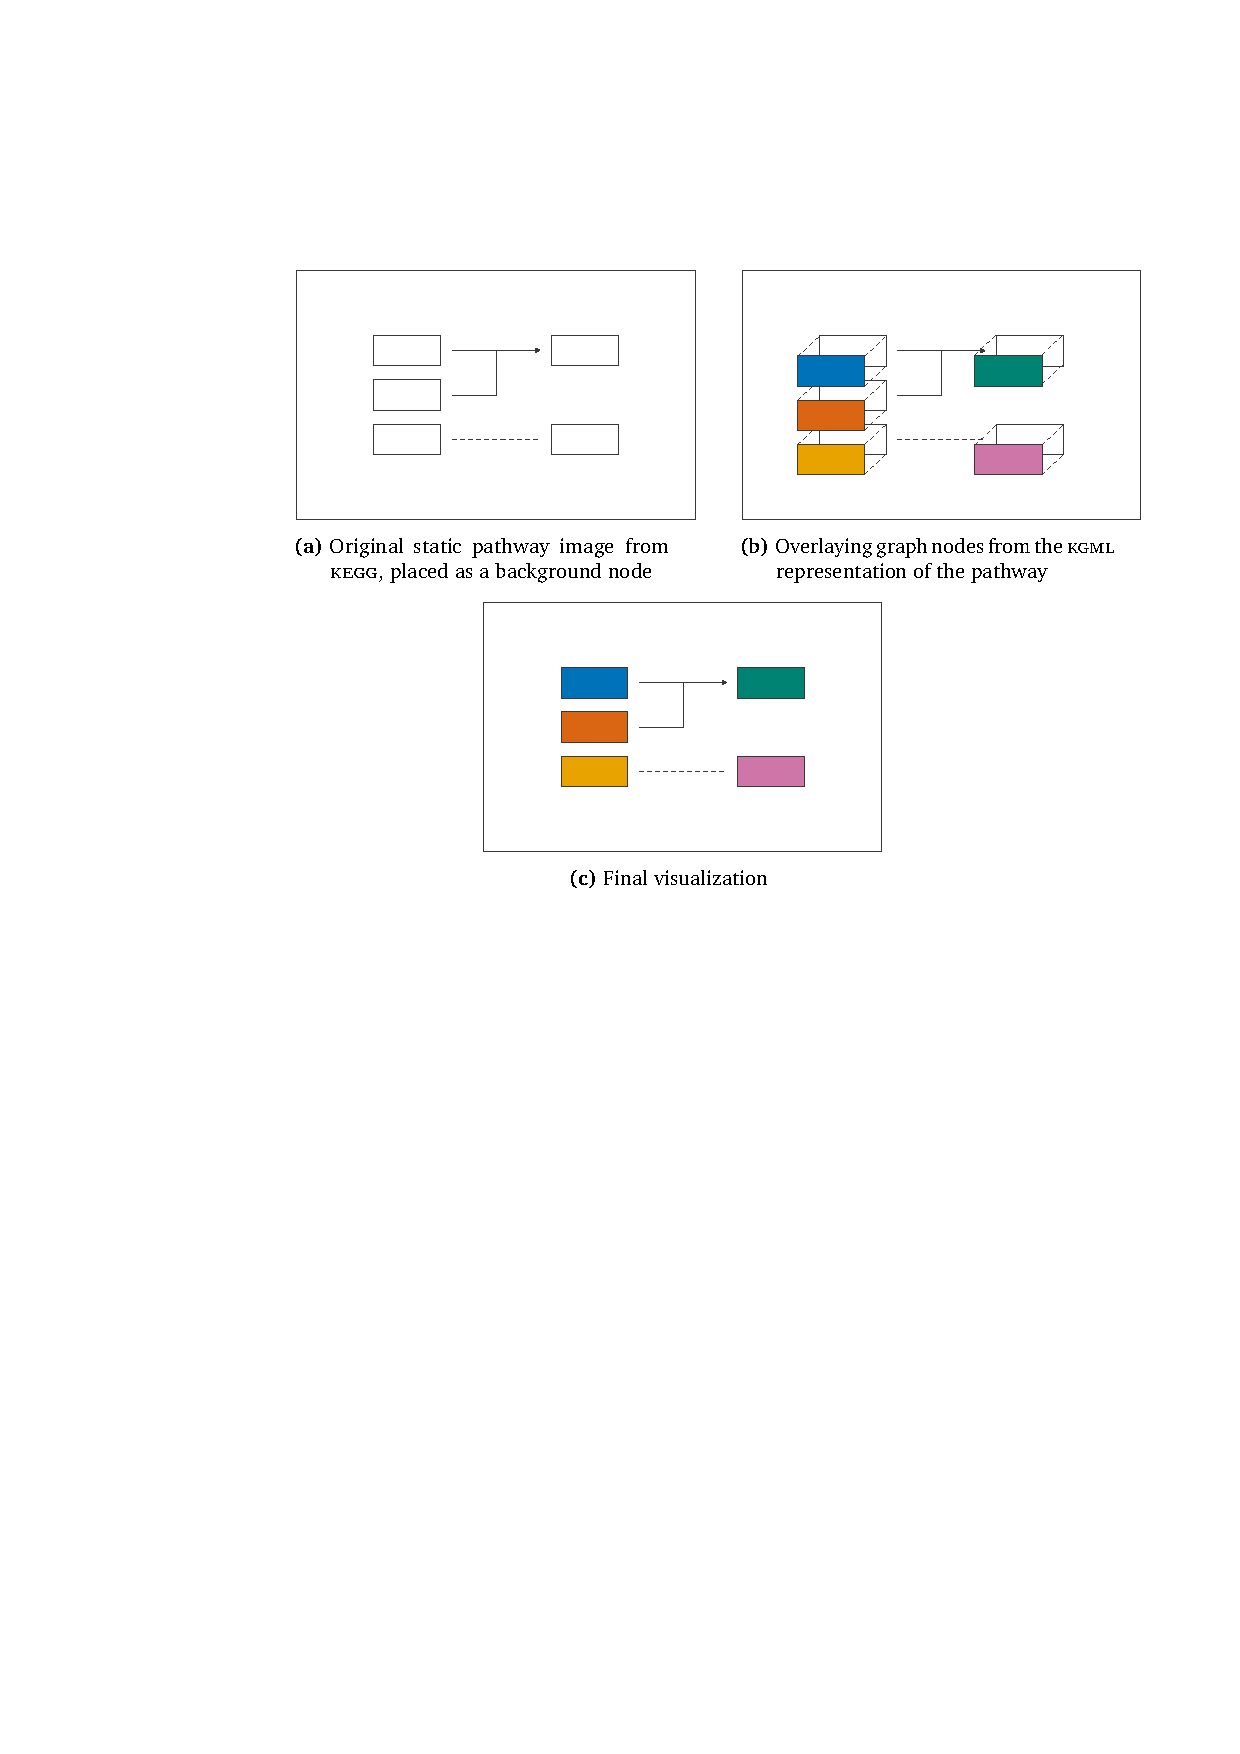
\includegraphics[width=\textwidth]{figures/how2pathway.pdf}
        \caption{Visualizing gene expression data on \gls{kegg} pathway maps.} 
    \label{fig:how2pathway}
    \end{centering} 
\end{figure}   

Kvik provides a flexible statistics backend where researchers can specify the
analyses they want to run to generate data for later visualization. For example,
in Kvik Pathways we retrieve fold change for single genes every time a pathway
is viewed in the application.  These analyses are run ad hoc on the backend
servers and generates output that is displayed in the pathways in the client's
web browser. The data analyses are implemented in an R script and can make use
of all available libraries in R, such as Bioconductor. 

Researchers modify this R script to, for example, select a normalization method,
or to tune the false discovery rate (FDR) used to adjust the $p$-values that
Kvik Pathways uses to highlight significantly differentially expressed genes.
Since Kvik Pathways is implemented as a web application and the analyses are run
ad hoc, when the analyses change, researchers get an updated application by
simply refreshing the Kvik Pathways webpage.

\subsection{Use Case: Analysis of Renin-Antiotensin Pathway}
As an example of practical use of Kvik Pathways, we chose one of the
significant pathways from the overlap analysis, the renin-angiotensin
pathway (Supplementary table S5 in \cite{olsen2013plasma}). The pathway
contains 17 genes, and in the pathway map we could instantly identify the
two genes that drive this result. The color of the gene nodes in the pathway
map indicates the fold change, and the statistical significance level is
indicated by the color of the node's frame.  We use this image of a
biological process to see how these two genes (and their expression levels)
are related to other genes in that pathway, giving a biologically more
meaningful context as compared to merely seeing the two genes on a list.

\section{Building Data Exploration Applications with Kvik}\label{kviksec}\label{challengeref} 
Through the experiences developing the Kvik Pathways we identified a set of
components and features that are central to building data exploration
applications: 

\begin{enumerate}
    \item A low-latency language-independent approach for integrating, or
        embedding, statistical software, such as R, directly in a data
        exploration application. 
    \item A low-latency language-independent interface to online reference
        databases in biology that users can query to explore results in context
        of results in context of known biology. 
    \item A simple method for deploying and sharing the components of an
        application between projects. 
\end{enumerate} 

We used these to design and implement Kvik which in turn formed the basis of  
the \gls{sme} approach that the \gls{mixt} web application builds upon. 

Kvik is a collection of software packages in the Go programming language. It is
designed for developers that want to develop interactive data exploration
applications. It is the foundation in our two data exploration applications, and
has been iteratively developed through the last years.\footnote{In \cite{fjukstad2015kvik} we refer to Kvik as \emph{Kvik Framework}, but we
have since shortened its name.}
Kvik provides an interface to the R statistical programming
language, both as a stand-alone service, a client library, and through an
OpenCPU server. It provides an R-based pipelining tool that allows useres to
specify and run statistical analysis pipelines in R.  Kvik also contains a
Javascript package for visualizing KEGG pathways using d3.\cite{d3}  In addition
it provides an interface with online databases such as MsigDB\cite{msigdb} and
\gls{kegg}\cite{kegg}.

We used the experience building Kvik Pathways to completely re-design and
re-implement the R interface in Kvik. From having an R server that can run a
set of functions from an R script, it now has a clean interface to call any
function from any R package, not just retrieving data as a text string but in a
wide range of formats. We also re-built the database interface, which is now a
separate service. This makes it possible to leverage its caching capabilities
to improve latency. This transformed the application from being a single
monolithic application into a system that consists of a web application for
visualizing biological pathways, a database service to retrieve pathway images
and other metadata, and a compute service for interfacing with the gene
expression data in the \gls{nowac} cohort. We could then re-use the database and the
compute service in the MIxT application. 

We have used these packages to develop the \gls{sme} approach through services
that provide open interfaces to the R programming language and the online
databases.  We outline these services in \ref{micrservices}.  In short the
interfaces are accessible through an HTTP interface and can be used from any
programming language.

\subsection{Design Priciples}\label{micrservices} 
We generalized our efforts from Kvik Pathways into the following design
principles for building applications in bioinformatics: 

\textbf{Principle 1}: Build applications as collections of language-agnostic
microservices. This enables re-use of components and does not enforce any
specific programming language on the user interfaces or the underlying
components of the application. 

\textbf{Principle 2}: Use software containers to package each service. This has
a number of benefits: it simplifies deployment, ensures that dependencies and
libraries are installed, and  simplifies sharing of services between
developers. 

\subsection{Compute Service}
We have built a compute service that provides an open interface directly to the
R programming language, thus providing access to a wealth of algorithm and
statistical analysis packages that exists within the R ecosystem.  
Application developers can use the compute service to execute specialized
analyses and retrieve results either as plain text or binary data such as plots.
By interfacing directly with R, developers can modify input parameters to
statistical methods directly from the user-facing application. 

The compute service offers three main operations to interface with R: i) to call
a function with one or more input parameters from an R package, ii) to get the
results from a previous function call, and iii) a catch-all term that both calls
a function and returns the results.  We use the same terminology as
OpenCPU\cite{opencpu} and have named the three operations Call, Get, and RPC
respectively. These three operations provide the necessary interface for
applications to include statistical analyses in the applications.

The compute service is implemented as an HTTP server that communicates with a
pre-set number of R processes to execute statistical analyses. 
At initiation of the compute service, a user-defined number of R worker sessions
are launched for executing analyses (default is 5).  
The compute service uses a round-robin scheduling scheme to distribute incoming
requests to the workers. We provide a simple FIFO queue for queuing of requests.
The compute service also provides the opportunity for applications to cache
analysis results to speed up subsequent calls. 

\subsection{Database Service} 
We have built a database service to interface with online biological databases.
The service provides a low latency interface, it minimizes the number of queries
to remote databases, and stores additional metadata to capture query parameters
and database information.  The database service provides an open HTTP interface
to biology databases for retrieving meta-data on genes and processes.  We
currently have packages for interfacing with E-utilities\cite{sayers2009entrez},
MSigDB, HGNC\cite{gray2014genenames}, and KEGG.

\section{\gls{mixt}}
The \gls{mixt} system is an online web application for exploring and comparing
transcriptional profiles from blood and tumor
samples.\cite{fjukstad2017building,dumeaux2017interactions} It provides users
with an interface to explore high-throughput gene expression profiles of breast
cancer tumor data with matched profiles from the patients blood. We have used
the microservices in Kvik to interface with statistical analyses and information
from online biology databases. 

\subsection{Analysis Tasks} 
To efficiently develop
the application we defined six analysis tasks (A1-A6) that the application
supports: 

\textbf{A1:} Explore co-expression gene sets in tumor and blood tissue.  Users
can explore gene expression patterns together with clinicopathological variables
(e.g. patient or tumor grade, stage, age) for each module.  In addition we
enable users to study the underlying biological functions of each module by
including gene set analyses between the module genes and known gene sets. 

\textbf{A2:} Explore co-expression relationships between genes. Users can
explore the co-expression relationship as a graph visualization. 
Here genes are represented in the network with nodes and edges represent 
statistically significant correlation in expression between the two end-points. 

\textbf{A3:} Explore relationships between modules from each tissue. We provide
two different metrics to compare modules, and the web application enables users
to interactively browse these relationships.  In addition to providing
visualizations the compare modules from each tissue, users can explore the
relationships, but for different breast cancer patient groups. 

\textbf{A4:} Explore relationships between clinical variables and modules. In
addition to comparing the association between modules from both tissues, users
also have the possibility to explore the association with a module and a
specific clinical variable. It is also possible to explore the associations
after first stratifying the tumors by breast cancer subtype (an operation that
is common in cancer related studies to deal with molecular heterogeneity).

\textbf{A5:} Explore association between user-submitted gene lists and computed
modules. We want to enable users to explore their own gene lists to explore
them in context of the co-expression gene sets. The web application must handle
uploads of gene lists and compute association between the gene list and the MIxT
modules on demand. 

\textbf{A6:} Search for genes or gene lists of interest. To facilitate faster
lookup of genes and biological processes, the web application provides a search
functionality that lets users locate genes or gene lists and show association to
the co-expression gene sets. 

\subsection{Architecture} 
We structured the MIxT application with a separate view for each analysis task.
To explore the co-expression gene sets (\textbf{A1}), we built a view that
combines both static visualizations from R together with interactive tables for
gene overlap analyses. Figure \ref{fig_first_case} shows the web page presented
to users when they access the co-expression gene set 'darkturquoise' from blood.
To explore the co-expression relationship between genes (\textbf{A2}) we use an
interactive graph visualization build with Sigma.\cite{sigmajs}
We have built visualization for both tissues, with graph sizes of 2705 nodes and
90 348 edges for the blood network, and 2066 nodes and 50 563 edges for the
biopsy network. 
To visualize relationships between modules from different tissues (\textbf{A3}),
or their relationship to clinical variables (\textbf{A4}) we built a heatmap
visualization.
We built a simple upload page where users can specify their gene sets
(\textbf{A5}). The file is uploaded to the web application which redirects it to
a backend service that runs the analyses. Similarly we can take user input to
search for genes and processes (\textbf{A6}).

\begin{figure}[h!]
\centering
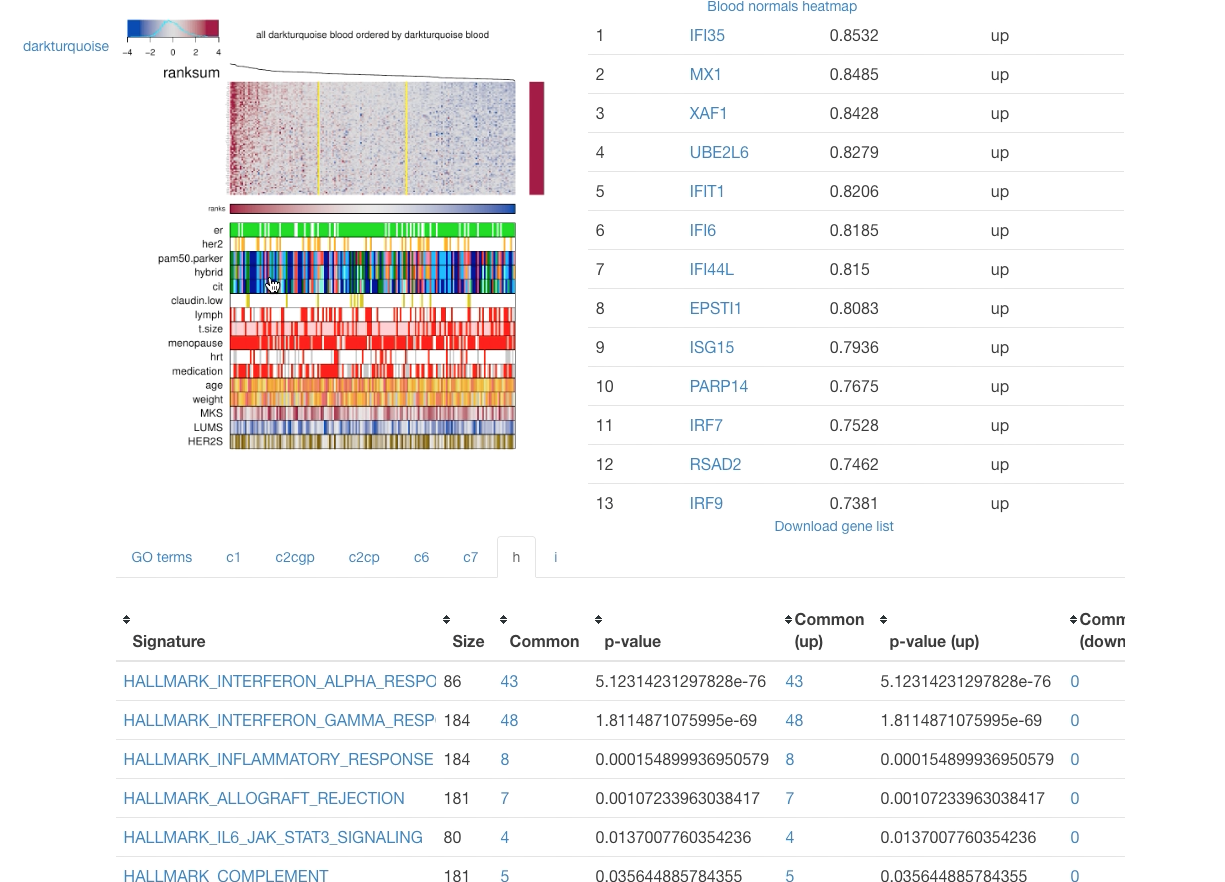
\includegraphics[width=\columnwidth]{figures/module.png}
    \caption[MIxT module overview page.]{MIxT module overview page.
The top left panel
contains the gene expression heatmap for the module genes. The top right panel
contains a table of the genes found in the module. The bottom panel contains the
results of gene overlap analyses from the module genes and known gene sets from
MSigDB.}
\label{fig_first_case}
\end{figure} 

For the original analyses we built an R package, mixtR,\footnote{Available
online at \url{github.com/vdumeaux/mixtR.}} with the statistical methods and
static visualizations for identifying associations between modules across
tissues. The mixtR package is based on the \gls{wgcna} R package to compute the
correlation networks\cite{langfelder2008wgcna}.  To make the results more easily
accessible we built a web application
that interfaces with the R package, but also online databases to retrieve
relevant metadata. To make it possible to easily update or re-implement parts of
the system without effecting the entire application, and we developed it using a
microservice architecture. The software containers allowed the application to be
deployed on a wide range of hardware, from local installations to cloud systems.

\subsection{Implementation} 
From the six analysis tasks we designed and implemented MIxT as a web
application that integrates statistical analyses and information from biological
databases together with interactive visualizations. Figure \ref{kvik-mixt} shows
the system architecture of MIxT which consists of three parts i) the
web application itself containing the user-interface and visualizations; ii) the
compute service performing the MIxT analyses developed in an R package,
delivering data to the web application; and iii) the database service providing
up-to-date information from biological databases.  Each of these components run
in Docker containers making the process of deploying the application simple. 

\begin{figure}[h!]
\centering
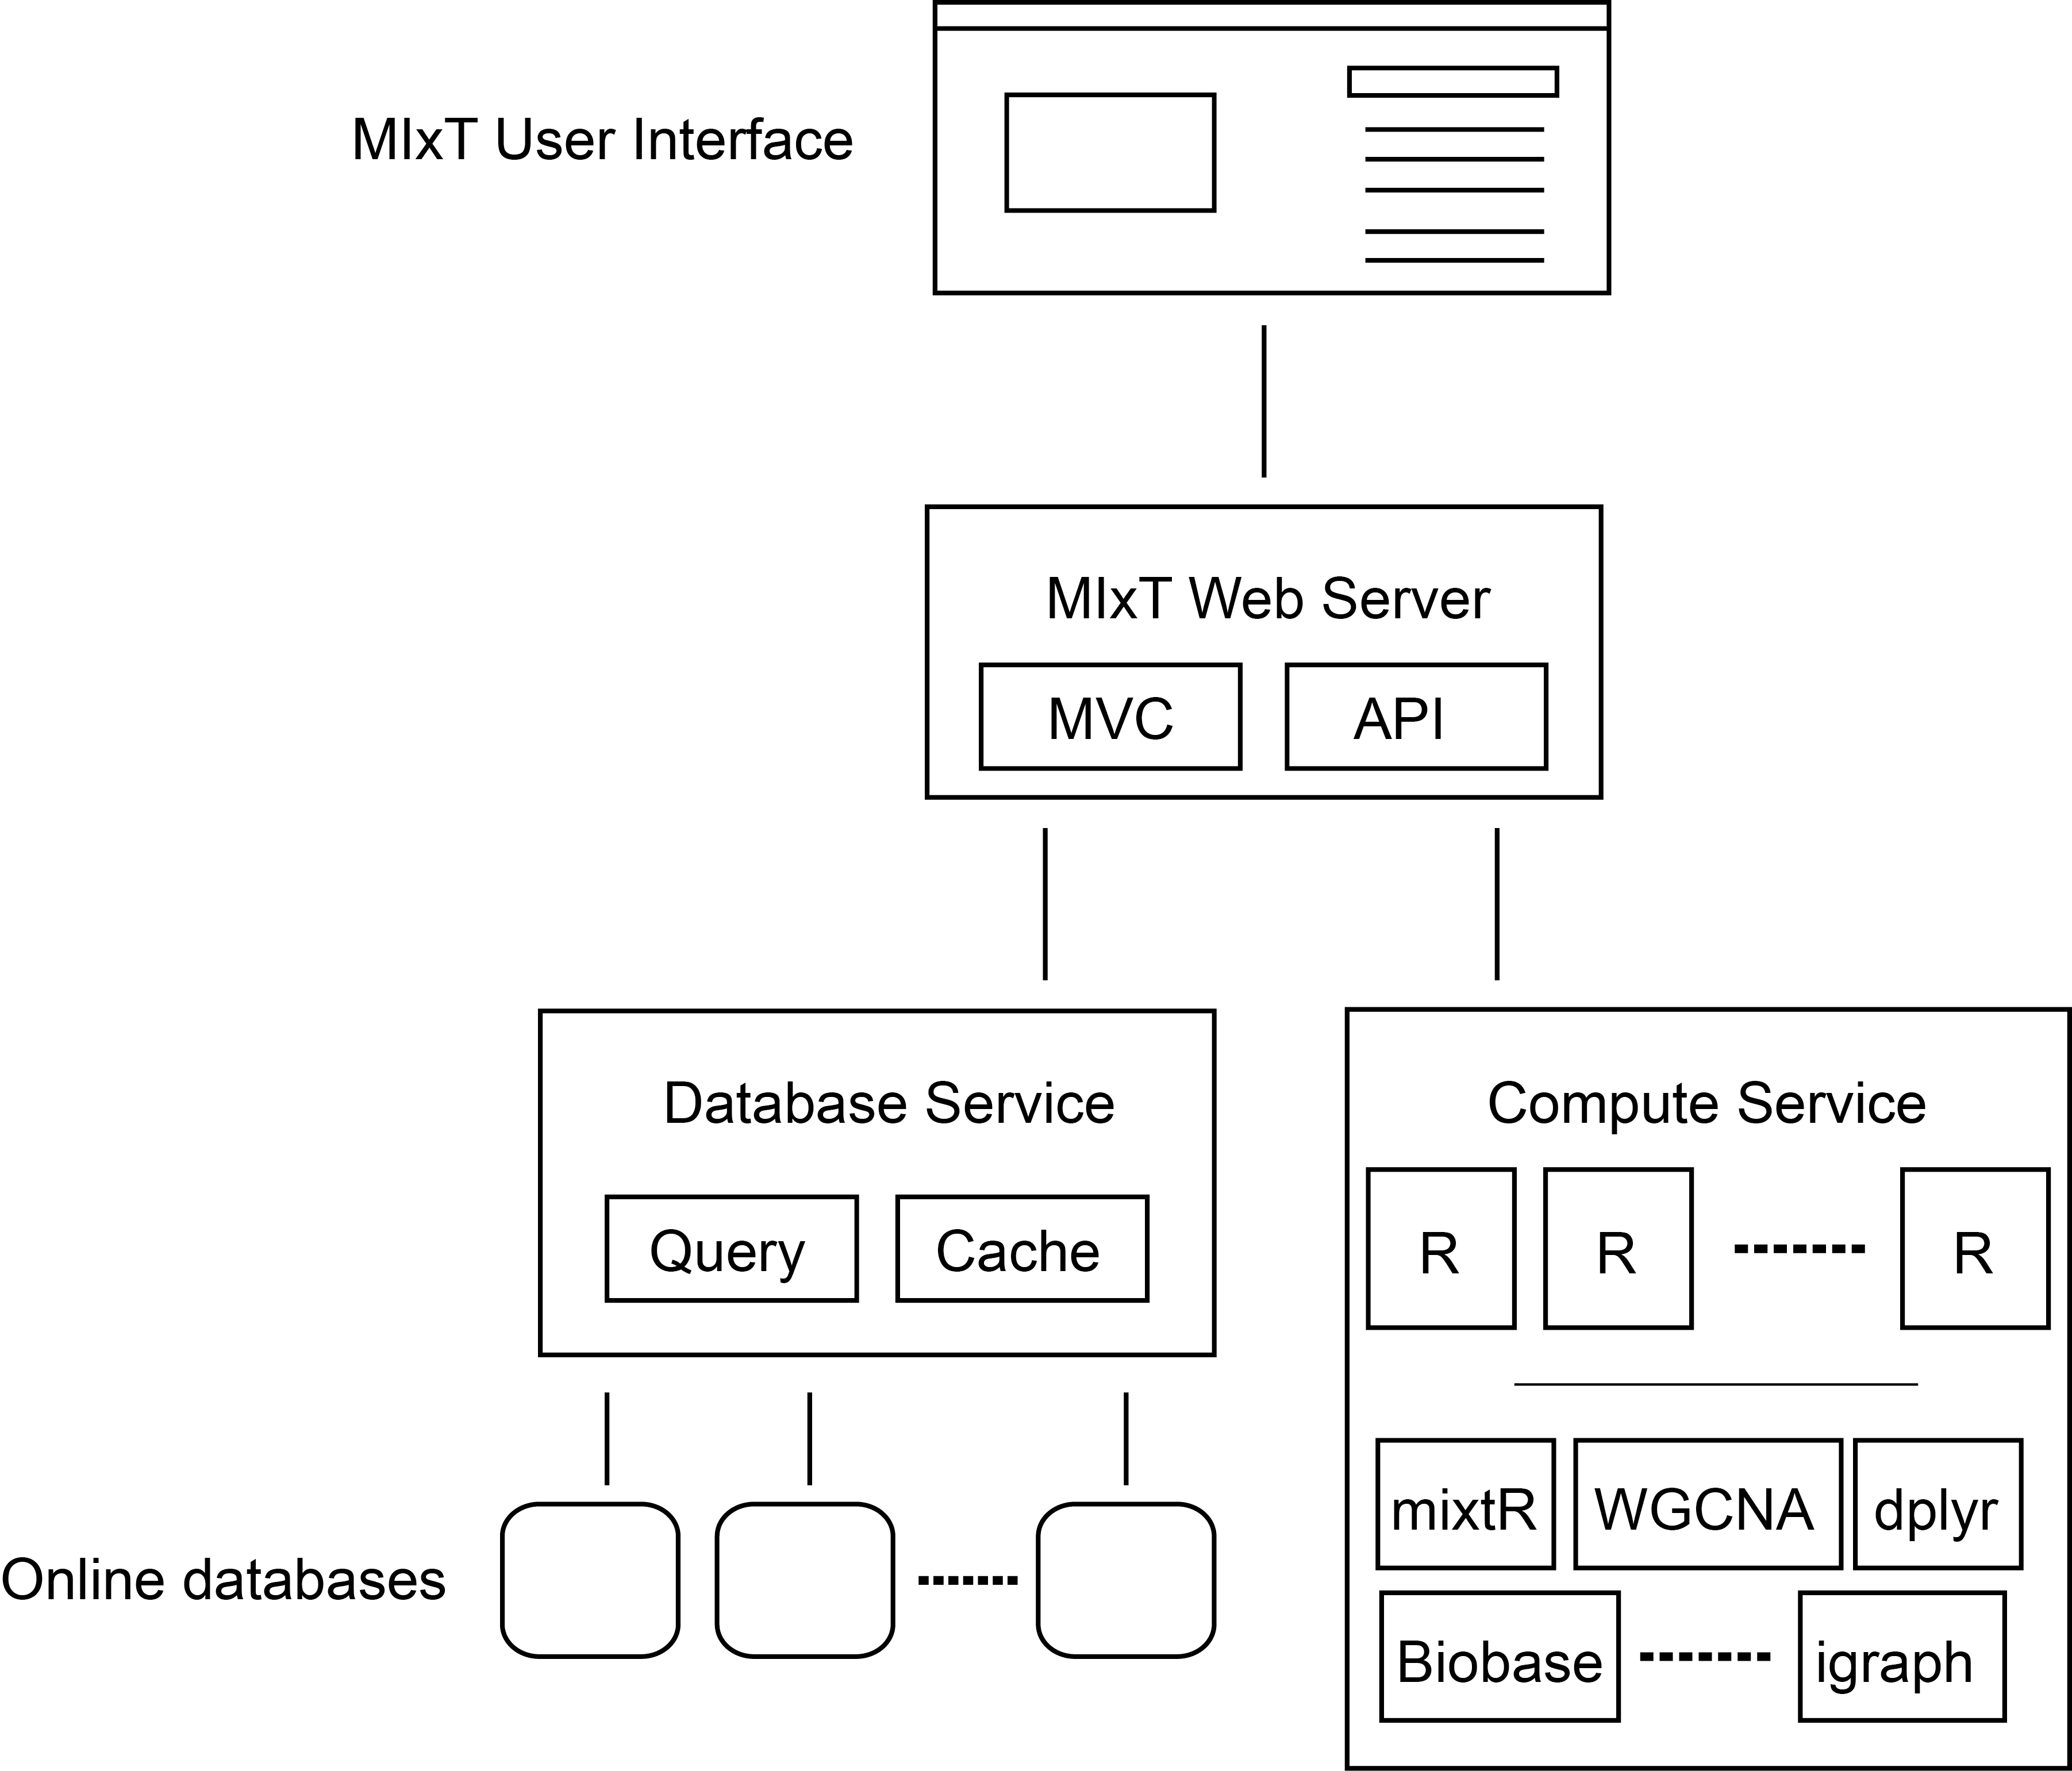
\includegraphics[scale=0.4]{figures/mixt-architecture.png}
    \caption[The architecture of the MIxT system.]{The architecture of the MIxT
    system. It consists of a web application, the hosting web server, a database
    service for retrieving metadata and a compute service for performing
    statistical analysis. Note that only the web application and the R package
    are specific to MIxT, the rest of the components can be reused in other
    applications.} 
\label{kvik-mixt}
\end{figure} 

The web application is hosted by a custom web server. This web server is
responsible for dynamically generating the different views based on data from
the statistical analyses and biological databases, and serve these to users. It
also serves the different JavaScript visualization libraries and style sheets. 

\subsection{Evaluation} 
We evaluate the MIxT application by investigating response times for a set of
queries to each of its two supporting services. 

To evaluate the database service we measure the query time for retrieving
information about a specific gene with and without caching.\footnote{More
details online at \url{github.com/fjukstad/kvik}.} This
illustrates how we can improve performance in an application by using a database
service rather than accessing the database directly. 
We use a AWS EC2 \emph{t2.micro}\footnote{See
\url{aws.amazon.com/ec2/instance-types} for more information about AWS EC2
instance types.} instance to host and evaluate the database service.  The
results in Table \ref{db} confirm a significant improvement in response time
when the database service caches the results from the database lookups. In
addition by serving the results out of cache we reduce the number of queries to
the online database down to one. 

\begin{table}[h]
\centering
    \caption{Time to retrieve a gene summary for a single gene, comparing
    different number of concurrent requests.}
    \begin{tabular}{| l | c | c | c | c | c | }
        \hline 
        & 1 & 2 & 5 & 10 & 15 \\ 
      \hline			
      No cache & 956ms & 1123ms & 1499ms & 2147ms & 2958ms\\
      \hline
      Cache & 64ms & 64ms & 130ms & 137ms & 154ms\\
      \hline  
    \end{tabular}
\label{db}
\end{table} 

We evaluate the compute service by running a benchmark consisting of two
operations: first generate a set of 100 random numbers, then plot them and
return the resulting visualization.\footnote{More details at
\url{github.com/fjukstad/kvik}.} We use two \emph{c4.large} instances on AWS EC2
running the Kvik compute service and OpenCPU base docker containers. The servers
have caching disabled.  Table \ref{kvikopencpucomparison} shows the time to
complete the benchmark for different number of concurrent connections. We see
that the compute service in Kvik performs better than the OpenCPU\footnote{Built
using the \textit{opencpu-server} Docker image.} alternative. We believe that
speedup is because we keep a pool of R processes that handle requests. In
OpenCPU a new R process is forked upon every request that results in any
computation executed in R. Other requests such as retrieving previous results do
not fork new R processes. 

In summary our results show that the interface to the R programming language
provides faster latencies, and that implementing a service for database lookups
have clear benefits with regards to latency. 

\begin{table}[h]
\centering
    \caption{Time to complete the benchmark with different number of
    concurrent connections.}
    \begin{tabular}{| l | c | c | c | c | c | }
        \hline 
       & 1 & 2 & 5 & 10 & 15 \\ 
      \hline			
      Kvik & 274ms & 278ms & 352ms & 374ms & 390ms\\
      \hline
      OpenCPU & 500ms & 635ms & 984ms & 1876ms & 2700ms\\
      \hline  
    \end{tabular}
\label{kvikopencpucomparison}
\end{table} 

\subsection{Tumor Epithelium-Stroma Interactions in Breast Cancer}
The MIxT web application is usable with other datasets as well. As already
mentioned, the web application retrieves datasets from an R package in a Kvik
compute service. If developers replace the datasets the web application will in
turn generate visualizations based on this data. Since we have open-sourced
every part of the system, application developers can download the respective
repositories where they will find instructions on how to deploy the system with
their own data. 

In addition to the MIxT web application for exploring the link between breast
tumor and primary blood, we have also deployed a web application that
investigates the link in another dataset.\cite{boersma2008stromal} We have
deployed the application online at \url{mixt-tumor-stroma.bci.mcgill.ca}. The
web application is identical, but the underlying dataset is different.

\subsection{air:bit}
We have also used the microservice architecture in an application where users
can upload and explore air pollution data from Northern
Norway.\cite{fjukstad2018low} In the project, air:bit, students from upper
secondary schools in Norway collect air quality data from sensor kits that they
have built and programmed. The web application lets the students upload data
from their kits, and provides a graphical interface for them to explore data
from their own, and other participating schools. The system consists of a web
server frontend that retrieves air pollution data from a backend storage system
to build interactive visualizations. It also integrates the data with other
sources such as the Norwegian Institute for Air Research and the The Norwegian
Meteorological Institute. 

\section{Related Work}\label{sec:int:rel}
There are different technologies for developing data exploration applications.
We have surveyed comparable applications for exploring similar datasets to the
ones we describe in this chapter, and underlying technology for developing these
applications. 

\subsection{Applications} 
There are a wealth of resources for exploring biological pathway maps.
\gls{kegg} provides a large collection of static pathway maps that users
can navigate through and download.\cite{kegg} They provide both static images of
the pathways, as well as a textual representation of the pathway in the
\gls{kgml}.  \gls{kegg} provides a \gls{rest} \gls{api} that developers can use
to integrate both pathway maps and other information in their application. In
\gls{kegg} Pathways we heavily rely on the data from \gls{kegg}.  Reactome is an
open-source peer-reviewed online knowledgebase of biomolecular
pathways.\cite{fabregat2018reactome} Users can download the entire graph
database or explore it in their pathway visualization tool. They have not yet
made an \gls{api} open for developers, but are planning to do so. Libraries such
as KEGGViewer\cite{villaveces2014keggviewer} allow developers to integrate
pathway visualization maps in web applications, but these are generated using
the \gls{kgml} representations, that do not include additional visual cues found
in the static \gls{kegg} pathway maps.  enRoute\cite{partl2012enroute} is a
desktop application for exploring pathway maps from \gls{kegg} that combines the
static pathway maps from \gls{kegg} in an interactive application. Pathview is
both an R package and an online web application for exploring pathway
maps.\cite{luo2017pathview} The online web application is built on top of the R
package and provides the same functionality, but through a \gls{gui}. Pathview
generates static pathway visualizations based on pathway maps from \gls{kegg}. 

There are few related systems that provide visualizations of the correlation
networks from \gls{wgcna}
results. The R package from the original paper provides a wide range of
different utility functions for visualization, but it is only accessible within
the R environment.  The \gls{wgcna} Shiny app\footnote{Online a
shiny.etriks.org/wgcna} is an interactive application for performing, and
exploring results from, \gls{wgcna}.  The online version allows users to explore
two demo datasets, and it is possible to download the application and change out
the datasets locally. In short it is a web implementation of the \gls{wgcna} R
package that allows users without any R experience perform \gls{wgcna}. It is
developed and maintained by the eTRIKS platform.\cite{bussery2018etriks}

\subsection{Technology} 
OpenCPU is a system for embedded scientific computing and reproducible
research.\cite{opencpu} Similar to the compute service in Kvik, it offers an
HTTP \gls{api} to the R programming language to provide an interface with
statistical methods. It allows users to make function calls to any R package and
retrieve the results in a wide variety of formats such as JSON or PDF. OpenCPU
provides a JavaScript library for interfacing with R, as well as Docker
containers for easy installation, and has been used to build multiple
applications.\footnote{\url{opencpu.org/apps.html}.}. The compute service in
Kvik follows many of the design patterns in OpenCPU. Both systems interface with
R packages using a hybrid state pattern over HTTP. Both systems provide the same
interface to execute analyses and retrieve results.  Because of the similarities
in the interface to R in Kvik we provide packages for interfacing with our own R
server or OpenCPU R servers.

Shiny is a web application framework for R\footnote{\url{shiny.rstudio.com}.}
It allows developers to build web applications in R without having to have any
knowledge about HTML, CSS, or Javascript. While it provides an easy alternative
to build web applications on top of R, it cannot be used as a service in an
application that implements the user-interface outside of R.  

Renjin is a JVM-based interpreter for the R programming language.\cite{renjin}
It allows developers to write applications in Java that interact directly with R
code. This makes it possible to use Renjin to build a service for running
statistical analyses on top of R. One serious drawback is that existing R
packages must be re-built specifically for use in Renjin. 

Cytoscape is an open source software platform for visualizing complex networks
and integrating these with any type of attribute
data.\cite{shannon2003cytoscape} Through a Cytoscape App, cyREST, it allows
external network creation and analysis through a REST \gls{api}\cite{ono2015cyrest},
making it possible to use Cytoscape as a service.  To bring the visualization
and analysis capabilities to the web applications the creators of Cytoscape have
developed Cytoscape.js\footnote{\url{js.cytoscapejs.org}.}, a JavaScript library
to create interactive graph visualizations.  Another alternative for biological
data visualization in the web browser is BioJS It provides a community-driven
online repository with a wide range components for visualizing biological data
contributed by the bioinformatics community.\cite{gomez2013biojs} BioJS builds
on node.js\footnote{\url{nodejs.org}.} providing both server-side and
client-side libraries. In MIxT we have opted to build the visualizations from
scratch using sigma.js and d3 to have full control over the appearance and
functionality of the visualizations. 

\section{Discussion}
In this chapter we have given a description of how we successfully built two
data exploration applications for high-throughput biological datasets. We have
iteratively developed these, and through our experiences we formed
an approach for developing such applications using disparate systems. 

The most clear distinction between our systems and the alternatives, is our
focus on integrating the user-facing visualizations with the underlying data
sources. We have put emphasis on this integration to allow users to thoroughly
investigate the underlying data behind the discoveries they make.  While some
systems, such as Shiny, allow developers to build web applications that maintain
this integration, it is not possible to interface with the analyses from outside
their system. With our approach in Kvik, we could have first implemented the
MIxT web application, before later developing an native desktop application that
re-used the same data interfaces. The main idea here is to create a platform
independent interface between the different parts that make up a data
exploration application, to facilitate reuse and transparency. With Kvik we
provide a language-independent interface between a data exploration application
and the underlying statistical analyses and online
databases. 

As we have seen in \ref{sec:int:rel} there are many applications that provide
the functionality to view and browse pathway maps, where most of which
use \gls{kegg} as its main data source. The applications then either reuse
the pathway maps, and augment them with gene expression data, or use the
underlying \gls{kgml} description and generate their own graphical
representation with gene expression data. Using the first method will provide
the additional visual ques found in the static pathway images, but the
visualizations are less flexible with regards to node and edge placement. Using
the second method provides more flexible graphs with regards to layout, but this
could make the visualizations less familiar to the users interpreting them. As
mentioned in \cite{o2018visualization}, familiar representations provide easier
to understand visualizations to the users. 

With both of these techniques the underlying gene expression datasets are
retrieved using different techniques. Most systems allow users to specify gene
expression values in some table format and render the values in top of the
pathway map.  These values are typically the end result of a long analysis
process which users have to track manually. By integrating the visualization
with the analysis software, typically R, it is possible to access data from
anywhere in the analysis process, and also provide detailed information to the
user regarding the underlying data analysis process.  What separates our
approach in Kvik Pathways to the other related systems, is this integration
between the end visualization and the gene expression datasets. By using Kvik it
is possible to develop applications that automatically lets users access the
underlying data analysis, and thereby connecting the interpretable end results
with the analyses. 

Of the related technologies, OpenCPU provides the most similar interface to
analyze datasets as the R interface in Kvik. While we started to explore OpenCPU
for use in our applications, we found through our benchmarking that it did not
provide satisfactory performance for our applications. It does however provide a
richer set of functionality, such as exporting data in many more formats and
running user-submitted scripts. We did not find it necessary for these additions
and implemented our own R interface that could provide the necessary interface
for us to implement data exploration applications. 

The \gls{wgcna} Shiny app provides similar visualizations as our MIxT web
application, but the application is limited to that of a web application. Shiny
lets its users develop applications written purely in R, including the backend
server and the user interfaces. In MIxT we developed an R package with a set of
resources, or endpoints, for application developers to access through a Kvik R
service. This allows application developers to develop the user-facing logic
using any type of technology or framework. The resources are available through
the HTTP API in Kvik making it possible for anyone to develop an
application on top of the dataset and analyses. We acknowledge the strength of R
for data analysis, but not for developing complex user-facing web applications. 

There are several advantages with reusing and sharing microservices over
libraries in bioinformatics applications, that would justify the cost of hosting
an maintaining a set of distributed microservices.
The most apparent disadvantage with microservices is having to
potentially orchestrate tens, or even hundreds, of services running in different
distributed environments. 
Container orchestration systems such as Kubernetes can help simplify this task,
but technical staff are still required to keep these systems operational. By
implementing a system using different microservices it will however become
possible for different research groups to share computational resources. In the
case of the MIxT web application, the compute service runs on a powerful compute
node, while the web application can run on a lightweight compute node. Other
applications that interface with R could have used our compute service, and would
not require the local resources to run and host it themselves. This could prove
valuable for institutions that do not have the required resources available.
Another argument for using a microservice approach is the possibility for using
different programming languages for each part of an application. This allows for
developers to use the best tools for each problem, e.g. R for biomedical data
analysis, and HTML and Javascript for interactive visualizations. 

\section{Future Work} 
We hope to continue development on applications for interactively exploring
biological datasets. Through our approach, and especially the interface to R, 
we are now able to develop applications that can use any function or retrieve
datasets from any R package. This includes the \texttt{nowac} package in
Chapter \ref{biodata}. We believe that there is a large potential in the
available datasets, and that researchers would benefit from being able to
interactively explore these. 

\subsection{MIxT} 
We intend to address few points in future work, both in the
MIxT web application as well as the supporting microservices.  The first issue
is to improve the user experience in the MIxT web application.  Since it is
executing many of the analyses on demand, the user interface may seem
unresponsive. We are working on mechanisms that gives the user feedback when the
computations are taking a long time, but also reducing analysis time by
improving the performance the underlying R package. The database service
provides a sufficient interface for the MIxT web application. While we have
developed the software packages for interfacing with more databases, these
haven't been included in the database service yet. In future versions we aim to
make the database service an interface for all our applications.  We also aim to
improve how we capture data provenance. We aim to provide database versions and
meta-data about when a specific item was retrieved from the database. 

One large concern that we haven't addressed in this chapter is security. In
particular one security concern that we aim to address in Kvik is the
restrictions on the execution of code in the compute service. We aim to address
this in the next version of the compute service, using methods such as
AppArmor\cite{apparmor} that can restrict a program's resource access. In
addition to code security we will address data access, specifically put
constraints on who can access data from the compute service.  We also aim to
explore different alternatives for scaling up the compute service.  Since we
already interface with R we can use the Sparklyr\cite{sparklyr} or
SparkR\cite{sparkr} packages to run analyses on top of
Spark.\cite{zaharia2012resilient} Using Spark as an execution engine for data
analyses will enable applications to explore even larger datasets.

\section{Conclusion}
We have designed an approach for building data exploration applications in
cancer research. We first implemented Kvik Pathways, a web application for
exploring a gene expression dataset in the context of pathway maps. We used our
experiences to generalize our efforts into a set of central components that
these types of applications require. Further we realized these in our \gls{sme}
approach implemented as a set of microservices.  Using these services we have
built a web application, MIxT, that integrates statistical analyses, interactive
visualizations, and data from biological databases. While we have used our
approach to build an application in cancer research, we believe that the
microservice architecture is suitable for data exploration systems in other
disciplines as well. This is because they can compose applications from
specialized tools and services required to visualize and analyze the different
possible datasets. 

In summary, our primary lesson learned from the experiences with develop our two
applications, is to compose and develop a data exploration system from
independent parts.  We chose to implement our systems using three separate
services. A compute service to provide statistical analyses, a database service
to provide access to biological databases, and the user interface. This makes it
possible to quickly re-implement parts of the system, but also allow others to
interface with its underlying components, not just the user interface. 
